\section{Registration Protocol}\label{sec:registration}
In this section, we describe a registration procedure followed by an advertiser to place an ad on a specific registrar. 
\subsection{Data Structures}
\para{Advertisement}
When advertisers send a registration request, they send an \emph{advertisement} (\emph{ad} in short). The ad contains the IP address of the advertiser, the ID of the advertiser, the topic the ad is for and additional information needed to later contact the advertiser (\eg an application-specific port number). In the remaining part of the paper, we omit the additional information for brevity. 

\para{Topic Table}
Registrars store received ads locally in a data structure called a \emph{topic table}. Each ad stored in the topic table has an associated expiry time, after which the ad is automatically removed. Once an ad is added to the table, the expiry time is set to a fixed value $a$. The topic table acts as a \emph{first in, first out} queue for ads. The total size of the topic table is limited by $C_\textit{topic\_table}$. \sysname does not impose topic/IP/ID-specific limits on the content of the \emph{topic table}. 
A single advertiser may place at most one ad for a specific topic in the topic table (registration requests for ads already in the table are ignored). However, advertiser may attempt to place ads for multiple topics at the same registrar.

\para{Ticket}
Tickets are immutable objects issued by registrars to advertisers when receiving a registration request. Each ticket contains:
\begin{itemize}
    \item Ad - repeated registration request (as described above). 
    \item Initial timestamp - the local time at the registrar when the ad was received for the first time, $t_\textit{init}$
    \item Waiting time - the waiting time calculated by the advertiser for the ad, $t_\textit{waiting}$. We describe the details on waiting time calculation in \Cref{sec:waitingTime}. 
\end{itemize}
The tickets are digitally signed by the issuing advertiser. 

\subsubsection{Registration Procedure}
An advertiser willing to register an ad at a registrar starts by sending an initial request containing uniquely its \emph{advertisement}. Based on the content of the topic table and the registration, the registrar calculates an ad-specific waiting time. The advertiser then issues a ticket including the calculated waiting time and the time of receiving the initial request and send it back to the advertiser. 

The advertiser waits for the indicated time and attempts to register again. The consecutive registration request must include the last ticket issued by the registrar. Tickets can be used uniquely during a registration window:
\begin{equation}\label{eq:registration_window}
    t_\textit{window} = [t_\textit{init} + t_\textit{waiting}, t_\textit{init} + t_\textit{waiting} + t_\textit{init} + \delta t_\textit{window}]
\end{equation}
All the registration requests outside the registration window are ignored by the advertiser. The registrar calculates the registration windows based on the content of the ticket. $\delta t_\textit{window}$ should be chosen to accommodate for the maximum delay between the advertiser and the registrar. 

The advertiser calculates a new waiting time, based on the current content of the topic table, every time it receives a registration request (with or without ticket). The waiting time in the ticket is used only to calculate the registration windows and prevent advertisers from trying register continuously. The ticket also allows to calculate an accumulated waiting time:
\begin{equation}
    t_\textit{cumulative} = \textit{now} - t_\textit{init}
\end{equation}
An ad is admitted iff the accumulated waiting time is equal or larger than the calculated waiting time $t_\textit{cumulative} \ge t_\textit{waiting}$\footnote{Note that a registration request without a ticket may be admitted directly if $t_\textit{waiting}=0$.}. For registration requests without a ticket $t_\textit{cumulative} = 0$. An advertiser that misses its registration windows (as specified by the most recent ticket), loses all its cumulative waiting time and must attempt to re-register without a ticket (\Cref{fig:ticket_validity}). Once an ad is admitted, the registrar confirms the registration to the advertiser. 

If the cumulative time is not sufficient, $t_\textit{accumulated} < t_\textit{waiting}$, the registrar issues a new ticket and the advertiser repeats the whole procedure. With consecutive registration attempts, advertisers increase their cumulative waiting time $t_\textit{cumulative}$ and eventually will be admitted. 



\begin{figure}
    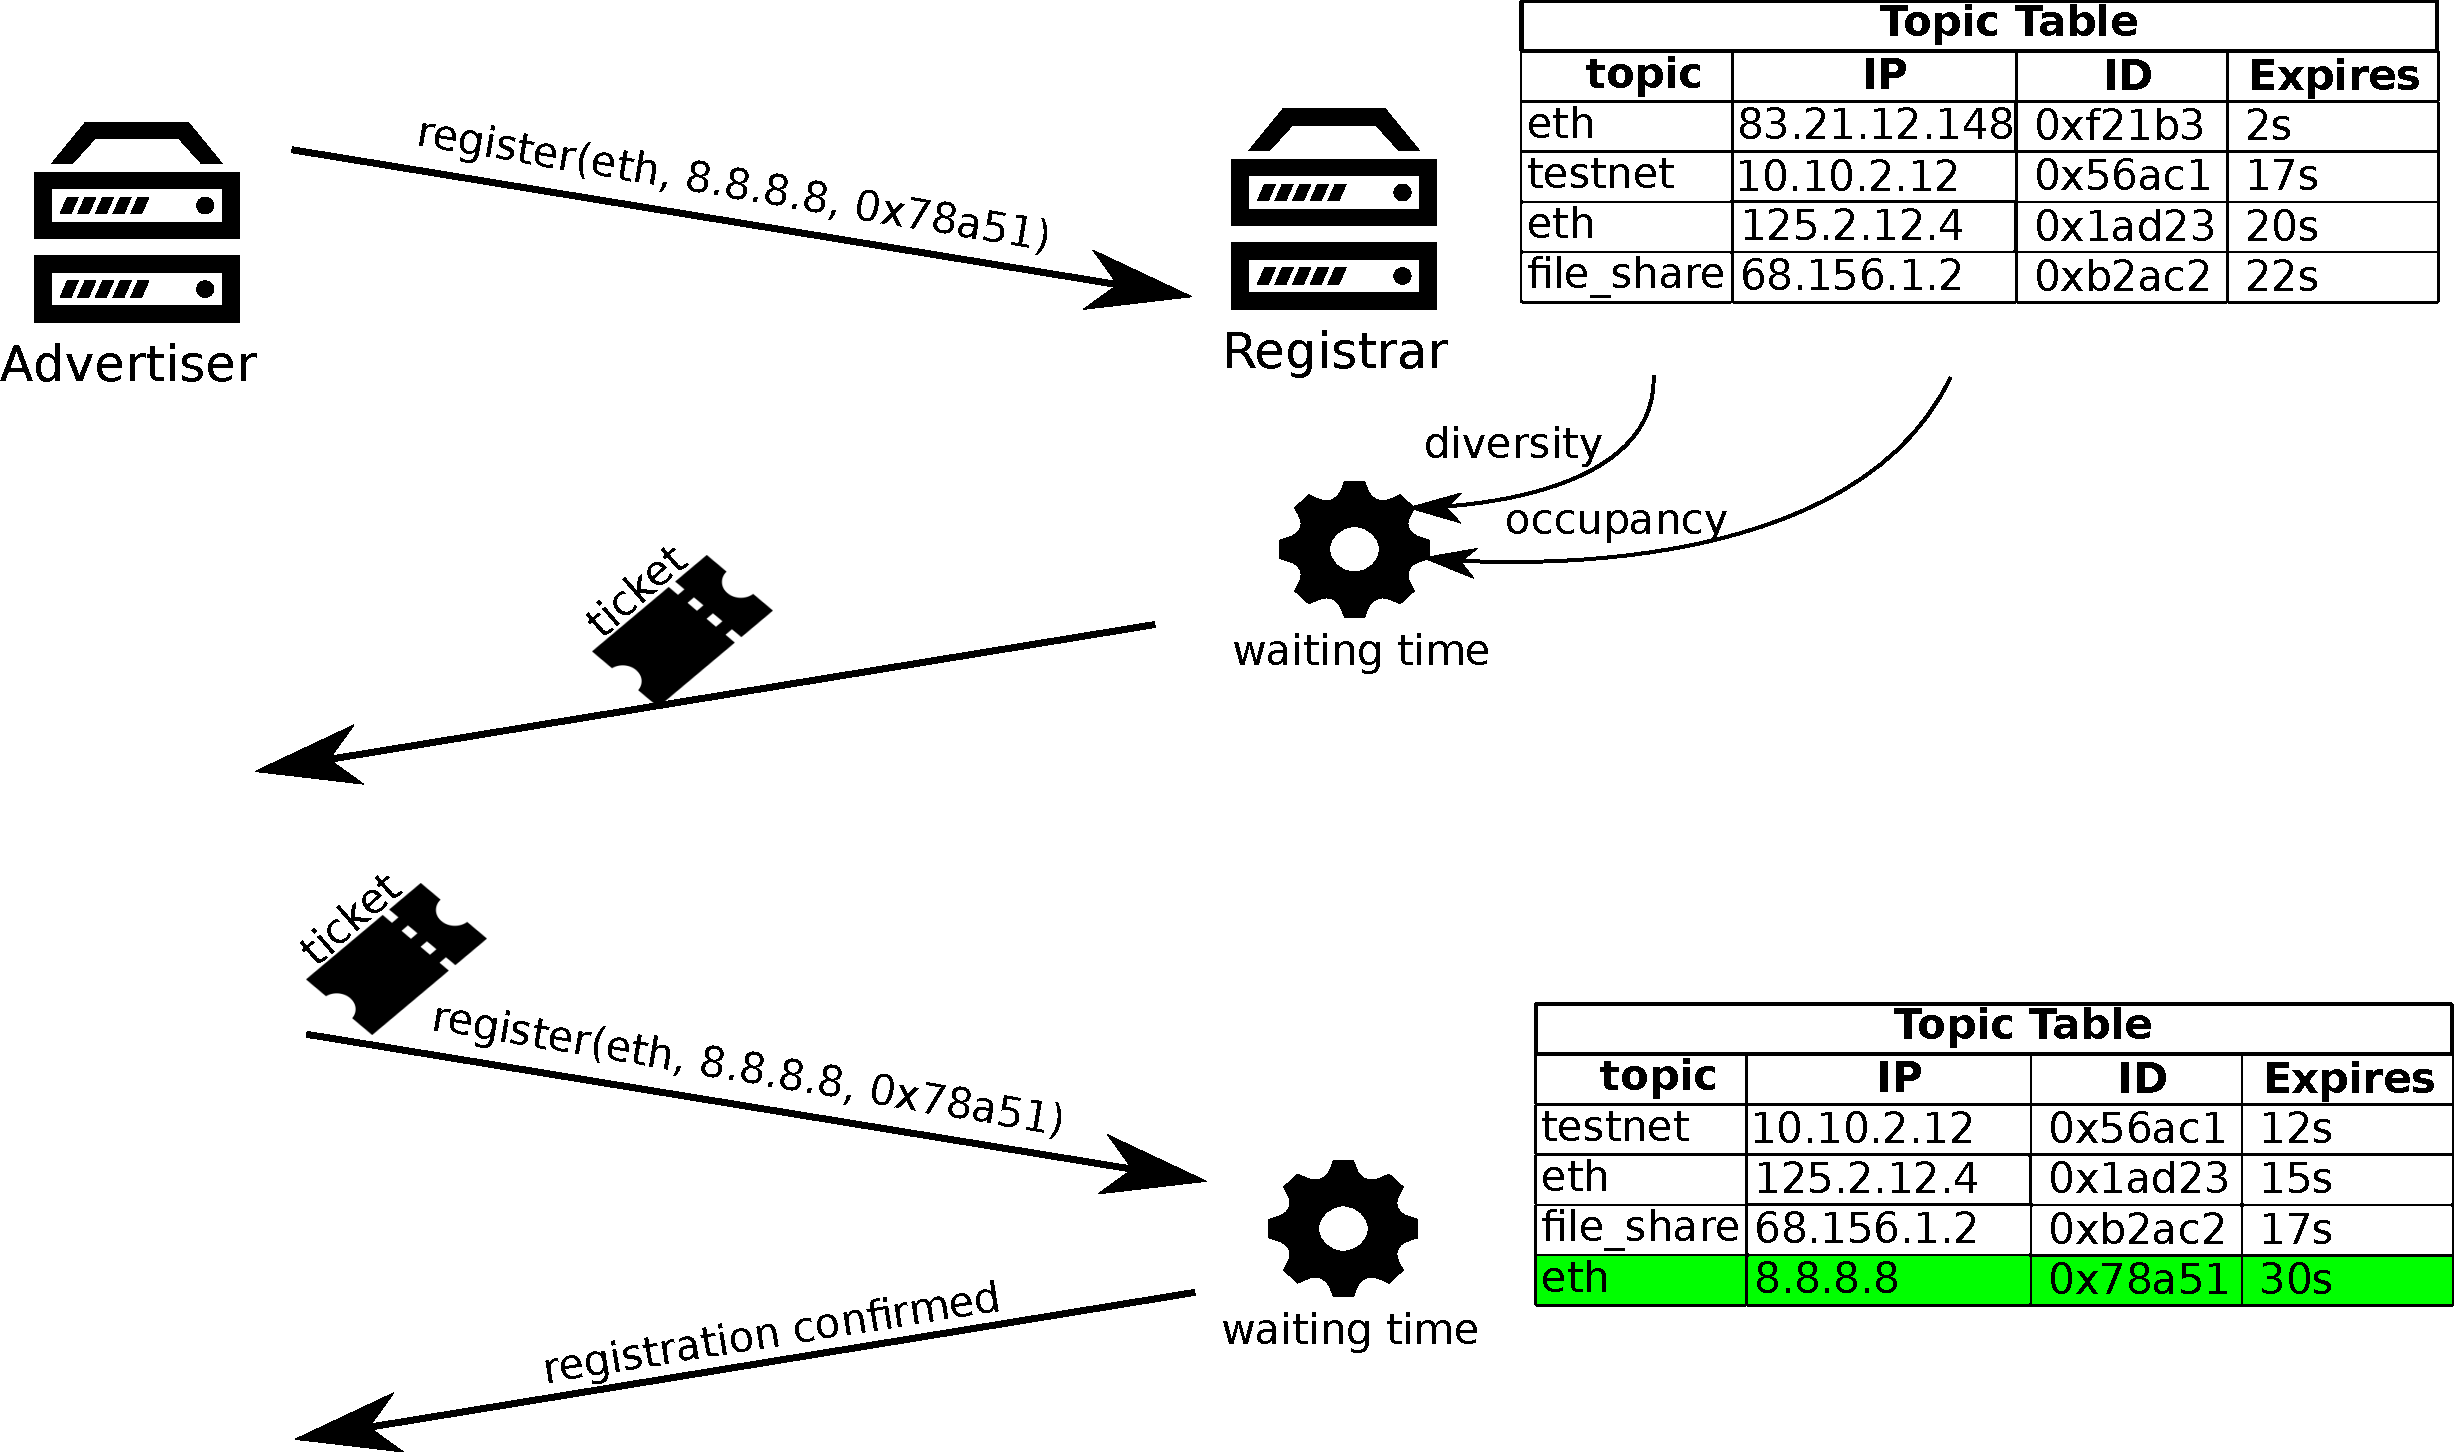
\includegraphics[width=0.5\textwidth]{img/registration}
    \caption{Registration operation.}
    \label{fig:registration}
\end{figure}

The inclusion of issue-time allows the registrars to prioritise advertisers that have been waiting the most as we explain later. Because the tickets are immutable (i.e., tampering with the ticket is detectable by the registrars that originally issued the ticket), when a registrar issues a new ticket (in case a registration is not immediately successful) to an advertiser, the registrar simply copies the issue-time from the last issued ticket and use that as the issue-time of the new ticket. This means that the registrars are not required to maintain any state for each on-going ticket request given that they can simply verify the authenticity of the ticket in the incoming registration requests. 


    
\begin{figure}
    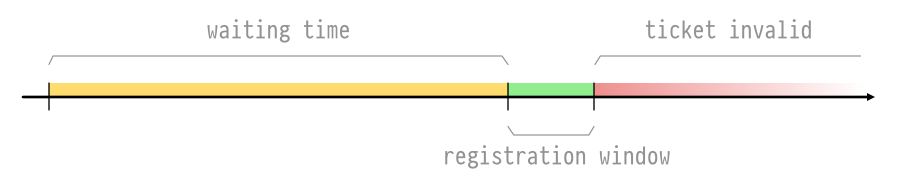
\includegraphics[width=0.5\textwidth]{img/ticket-validity}
    \caption{Ticket validity period.}
    \label{fig:ticket_validity}
\end{figure}

An advertiser gives up and stops the registration process with a registrar upon either $r$ unsuccessful registration attempts (i.e., after being issued $r$ tickets without being admitted. In that case, the advertiser removes the registrar from its registration table and selects a new node located in the same bucket and attempts a new registration procedure. 
%\michal{Is the below true? Shouldn't we try to register at the same node?}
%\sergi{We dont use the same, we pick another randomly. we could use the same but i think for diversity could be better  this way}
Similarly,  after the expiration of a previously placed ad the node is removed from the ticket table and the process is restarted with a new node picked from the local table.
\ramin{Confirmation message contains expiration time?}
\michal{Good point. We assumed a common expiration time so didn't include it in the response. But it might be good to either clarify that or include the expiration time in the response.}

%\michal{We're mixing here single-registrar registration process. It should be covered in the first section.}
%In our approach,  advertisers start a limited number of parallel registrations in each ticket table bucket distance.
% More specifically, an advertiser follows the below steps to distribute its ads for a specific topic:
%\begin{enumerate}
     %\item The advertiser (\hl{randomly?}) selects a set of K registrar nodes from each bucket distance of the ticket table structure, where the number of bucket distances (B) is a configurable parameter of the ticket table.
%    \item The advertiser selects a K random of node.,  by querying the local Ethereum routing table,  for each bucket distance.
    %\item A TICKETREQUEST message is initially sent to each of the selected registrar nodes in the previous step.
%    \item Registrar node replies with a TICKETRESPONSE.  This message includes the TICKET which contains a waiting time and a ticket issue time.  The TICKET is stored in the table.
    %\item The advertiser replies after the waiting time expires with a REGTOPIC request containing the previously received TICKET attached to it.
    %\item After the TICKET reception the waiting time is calculated again at the registrar.  A registration is successful when the waiting time calculated at the registrar is smaller than the cumulative waiting time,  which means that the advertiser has waited long enough.
    %\item The registrar sends a REGCONFIRMATION response to the advertiser of the successful registration. In general, the topic table occupancy is guaranteed to always remain below the topic table capacity by the waiting time calculated: the waiting time function returns increasingly large values as the topic table space runs out; the waiting time becomes infinite in case there is no space.
    %\item In case the new calculated waiting time is not smaller than the cumulative waiting time, the registration is not successful and the registrar replies with a REGRESPONSE message containing a new TICKET (containing a new waiting time).
    %\item 
%\end{enumerate}



%Reasonable \texttt{topic table capacity} is 50,000 ads. 
%Since ENRs are at most 300 bytes in size, these limits ensure that a full topic table consumes approximately 15MB of memory.
%The topic table is shared across multiple advertisers and stores topics with varying popularity (which is determined by how many nodes register the topic) among the participants of \sysname. 
%It is important that the high popularity of a particular topic should not prevent peers from registering less popular topics. 
%This is achieved using the waiting time function that will determine the time an advertiser will have to wait to place an ad after a ticket request,  and is detailed in Section~\ref{sec:waitingTime}.



%storing arbitrary information determined by the issuing registrar node.  While details of encoding and ticket validation are up to the implementation, tickets must contain enough information to verify that:
%\begin{itemize}
%    \item The advertiser attempting to use the ticket is the one which originally requested it.
%    \item A ticket is valid for a single topic only.
%    \item A ticket can only be used within the 'registration window' (explained below).
%    \item A ticket can not be used more than once.
%\end{itemize}

%In addition to the waiting time,  the sequence of tickets issued by a registrar for a specific advertiser also records the original issue-time of the first ticket which can be used to compute the cumulative waiting time so far; that is, the time elapsed since the advertiser requested its first ticket to place its ad. 



%\michal{Change the markdown notation of variables (CAPACITY) to scientific (n)}
%Any REGTOPIC messages that are not sent during the registration window determined by the waiting time (indicated in the ticket),   (as seen in Figure \ref{fig:ticket_validity}) are ignored by the registrars.  
%If the advertiser comes back during the established registration window,  the advertiser can either place the ad (and notify the advertiser of a successful registration) or issue another ticket with a new waiting time in another ticket response message. 
%An advertiser may be given one or more tickets in a sequence before a successful registration,  and this means that overall the advertiser waits for a 'cumulative waiting time' period that is the sum of multiple waiting times issued in each ticket in the sequence before finally registering an ad. 
%Assignment of 'waiting times' is the only way the registrars can control the registrations in order to both:

%\begin{itemize}
%    \item Throttle ad placement rate to prevent overflowing of topic table: when the topic table is full, the advertisers must wait for already placed ads to expire first before they are allowed to register new ads.
%    \item Prioritise registrations to achieve a diverse set of ads in the topic table. For example, registrations for less popular topics or registrations from advertisers that increase IP diversity (in the set of advertiser IP addresses that currently have an ad in the table) can be prioritised over others. This is useful to reduce the impact of Sybil attacks on the service discovery system.
%\end{itemize}

%Waiting times will be calculated according to a 'Waiting time function' detailed in Section~\ref{sec:waitingTime}.  Enforcing this time limit prevents misuse of the topic table because any topic must be important enough to outweigh the cost of waiting for ad placement. Imagine a group phone call: announcing the participants of the call using topic advertisement isn't a good use of the system because the topic exists only for a short time and will have very few participants. The waiting time prevents using the topic table for this purpose because the call might already be over before everyone could get registered. Also, it prevents attackers from overflowing topic table by regulating registrations in case of spamming attacks.



%The registrars ensure the authenticity of the tickets they issue to the advertisers through symmetric encryption we explain below.
